\documentclass[aspectratio=43,unicode]{beamer}
\usetheme{Moscow}

\usepackage[utf8]{inputenc}
\usepackage[T2A]{fontenc}
\usepackage[main=russian,english]{babel}

\usepackage{amsmath,amssymb}
\renewcommand{\thefootnote}{\fnsymbol{footnote}}

\hypersetup{
	pdfauthor={Ivan Tsybulin}
}

\usepackage{euler}

\graphicspath{{images//}}

\title[Погрешности. Дифференцирование]{Погрешности вычислений\\Численное дифференцирование}
\author[Цыбулин Иван]{\texorpdfstring{Скалько Юрий Иванович\\\textbf{Цыбулин
Иван}}{Цыбулин Иван}}
\date{}

\newcommand{\colorhref}[2]{\href{#1}{\textcolor{miptbase!30!black}{#2}}}

\begin{document}

\begin{frame}[plain]
  \titlepage %
\end{frame}

\section{}
\subsection{}

\begin{frame}
	\frametitle{Материалы по курсу вычислительной математики}
	\begin{itemize}
		\item Материалы курса (методички, лекции, учебники и др.) можно найти
			на \colorhref{http://crec.mipt.ru/study/materials/compmath/}
			{сайте кафедры вычислительной математики}
		\item
		Любые вопросы по курсу (и не только) можно присылать на почтовый ящик
		\colorhref{mailto:tsybulin@crec.mipt.ru}{tsybulin@crec.mipt.ru}
\end{itemize}
\end{frame}

\section{Погрешности}
\subsection{Виды погрешностей}
\begin{frame}
\frametitle{Абсолютная и относительная погрешность}
Если про величину $X$ известно, что $X \in [\bar{X}-\frac{\Delta X}{2}, \bar{X}+\frac{\Delta X}{2}]$, то
\begin{itemize}
	\item \emph{абсолютной погрешностью} $X$ называется величина $\Delta X$
	\item \emph{относительной погрешностью} --- отношение $\frac{\Delta X}{\left|\bar{X}\right|}$
\end{itemize}
\end{frame}

\subsection{Простейшие вычислительные задачи}
\begin{frame}
\frametitle{Приближенные вычисления}
\begin{block}{Задача}
	Как вычислить сложную функцию (например, $f(x) = \sin x$) в некоторой заданной точке?
\end{block}

\begin{itemize}
	\pause \item Воспользоваться большой таблицей заранее посчитанных значений функций
	\pause

	\alert{Но ведь эту таблицу необходимо еще составить!}
	\alert{Не ясно, как искать значения, которые в таблице отсутствуют}
	\pause \item Численно решить дифференциальное уравнение $y''(x) + y(x) = 0$
	\pause

	\alert{Пока совершенно не ясно, как это сделать (но это только пока!)}
	\pause \item Воспользоваться представлением в виде рядов
	\pause

	\textcolor{green!50!black}{Простейший вариант --- воспользоваться рядом Тейлора}
\end{itemize}
\end{frame}

\begin{frame}
\frametitle{Ряд Тейлора}
	Для функции $\sin x$ ряд Тейлора в окрестности точки $x=0$ выглядит следующим образом
	\[
	\sin x = x - \frac{x^3}{6} + \frac{x^5}{120} + \dots = \sum_{k=0}^{\infty} (-1)^k\frac{x^{2k+1}}{(2k+1)!}
	\]
	\pause
	\begin{block}{Вопрос}
	Какой радиус сходимости этого ряда?
	\pause

	$R = \infty$, Ряд сходится при любом $x \in \mathbb{C}$
	\end{block}
	\begin{itemize}
	\pause\item Но как суммировать бесконечный ряд на практике?
	\pause\item Ограничимся только несколькими членами этого ряда
	\pause\item Необходимо оценить ошибку, допущенную при этом
	\end{itemize}
\end{frame}

\subsection{Приближенные методы}
\begin{frame}
\frametitle{Практический метод}
	Итак, для приближенного вычисления $\sin x$ можно просуммировать
	несколько первых членов ряда Тейлора. Для оценки ошибки воспользуемся
	формулой Тейлора с остаточным членом в форме Лагранжа

	\[
	\sin x = \underbrace{\sum_{k=0}^{n} (-1)^k \frac{x^{2k+1}}{(2k+1)!}}_{S_n} +
	\frac{x^{2n+2}}{(2n+2)!}\sin^{(2n+2)} \xi,
	\quad \xi \in [0, x]
	\]

	\pause

	Отбросив остаточный член, мы тем самым допускаем ошибку
	\[
	\varepsilon_{\text{метод}}\equiv
	\left|\frac{x^{2n+2}}{(2n+2)!}\sin^{(2n+2)} \xi \right| \leqslant
	\frac{x^{2n+2}}{(2n+2)!}M_{2n+2}
	\]
	Здесь для максимума модуля $2n+2$-й производной использовано стандартное в
	вычислительной математике обозначение $M_{2n+2}$.
\end{frame}

\begin{frame}
\frametitle{Погрешность метода}
	Ошибка $\varepsilon_{\text{метод}}$ обусловлена тем, что метод, который мы
	применяем для вычисления значения функции, является \emph{неточным}.
	Данная ошибка называется \emph{ошибкой метода} (или \emph{погрешностью метода})

	\pause

	Так как все производные функции $\sin x$ ограничены по модулю единицей, $M_{2n+2} = 1$ и
	\[
	\varepsilon_{\text{метод}} = \frac{x^{2n+2}}{(2n+2)!}
	\]
	При стремлении $n \rightarrow \infty$ ошибка метода начиная с $n = n_0 >
	x/2$ монотонно стремится к нулю.
\end{frame}

\begin{frame}
\frametitle{Погрешность метода}
	Для знакопеременных рядов, члены которого монотонно убывают по модулю
	(начиная с некоторого $n_0$) справедлива следующая
	\begin{block}{Теорема}
	Сумма <<хвоста>> монотонно убывающего знакопеременного ряда не
	превосходит по модулю модуля первого слагаемого в <<хвосте>>.
	\end{block}

	Из этой теоремы сразу следует, что ошибка метода (сумма отброшенного
	<<хвоста>> ряда) при суммировании ряда для
	синуса не превосходит
	\[
		\varepsilon_\text{метод} \leq \frac{x^{2n+3}}{(2n+3)!}.
	\]
	Данная оценка не содержит максимумов производных, и, поэтому, удобнее на
	практике для сложных функций.
\end{frame}

\subsection{Численные эксперименты}
\begin{frame}
\frametitle{Проверка}
	Для проверки посчитаем $\sin \frac{\pi}{2}$ суммируя до $50$ членов ряда.

	\begin{figure}%
	\centering
	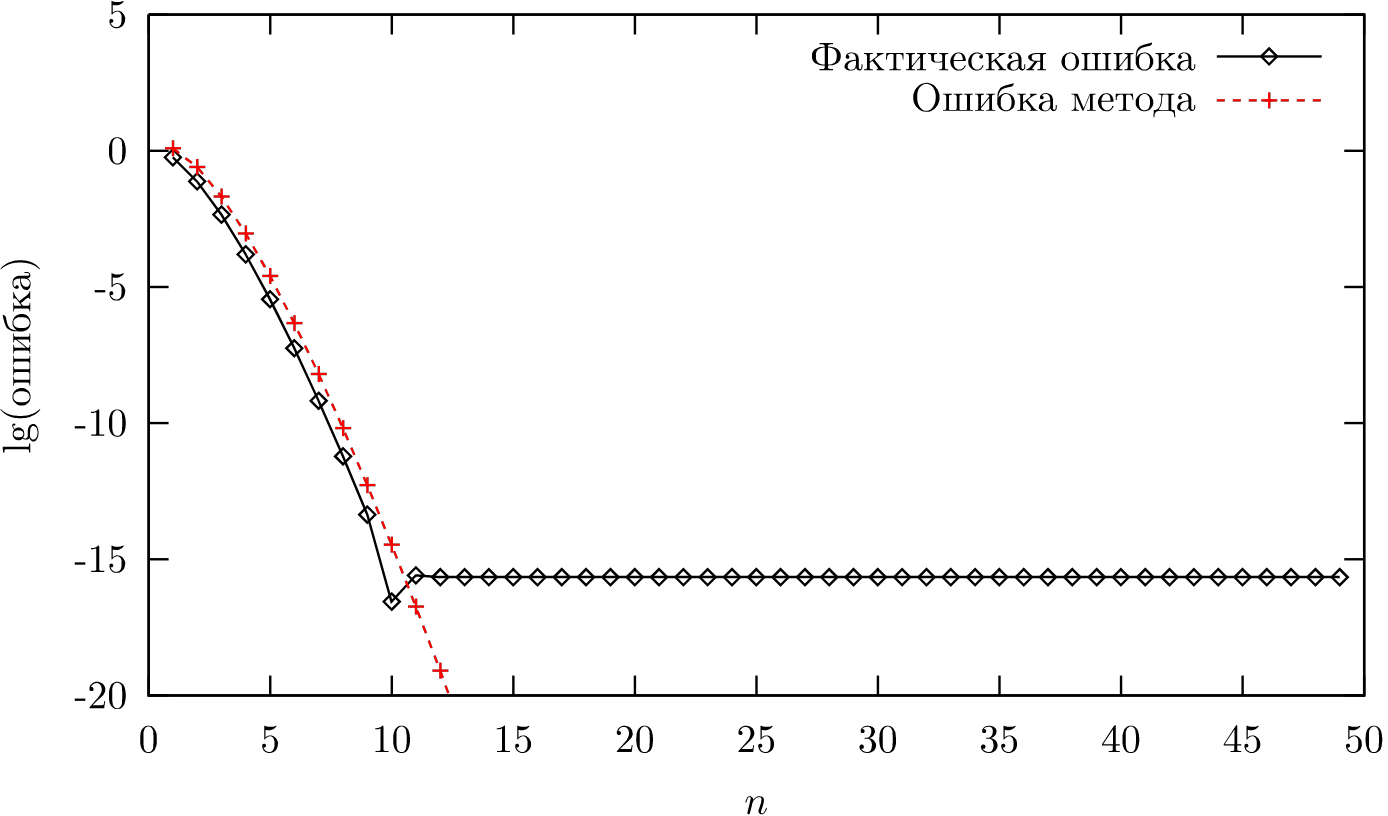
\includegraphics[height=0.4\textheight]{sine_pi_2.png}
	\end{figure}

	После сложения $10$ членов ряда фактическая ошибка составила $10^{-16}$ и перестала уменьшаться.
	Такое поведение говорит про наличие еще какой-то погрешности, кроме ошибки метода.
	\begin{block}{}
	Но ведь $10^{-16}$ это же совсем немного? Или нет?
	\end{block}
\end{frame}

\begin{frame}
\frametitle{Проверка №2}
	Проделаем аналогичные вычисления, но уже для $\sin \frac{17\pi}{2}$
	\footnote{$x = \frac{17\pi}{2} \approx 26.7$}

	\begin{figure}%
	\centering
	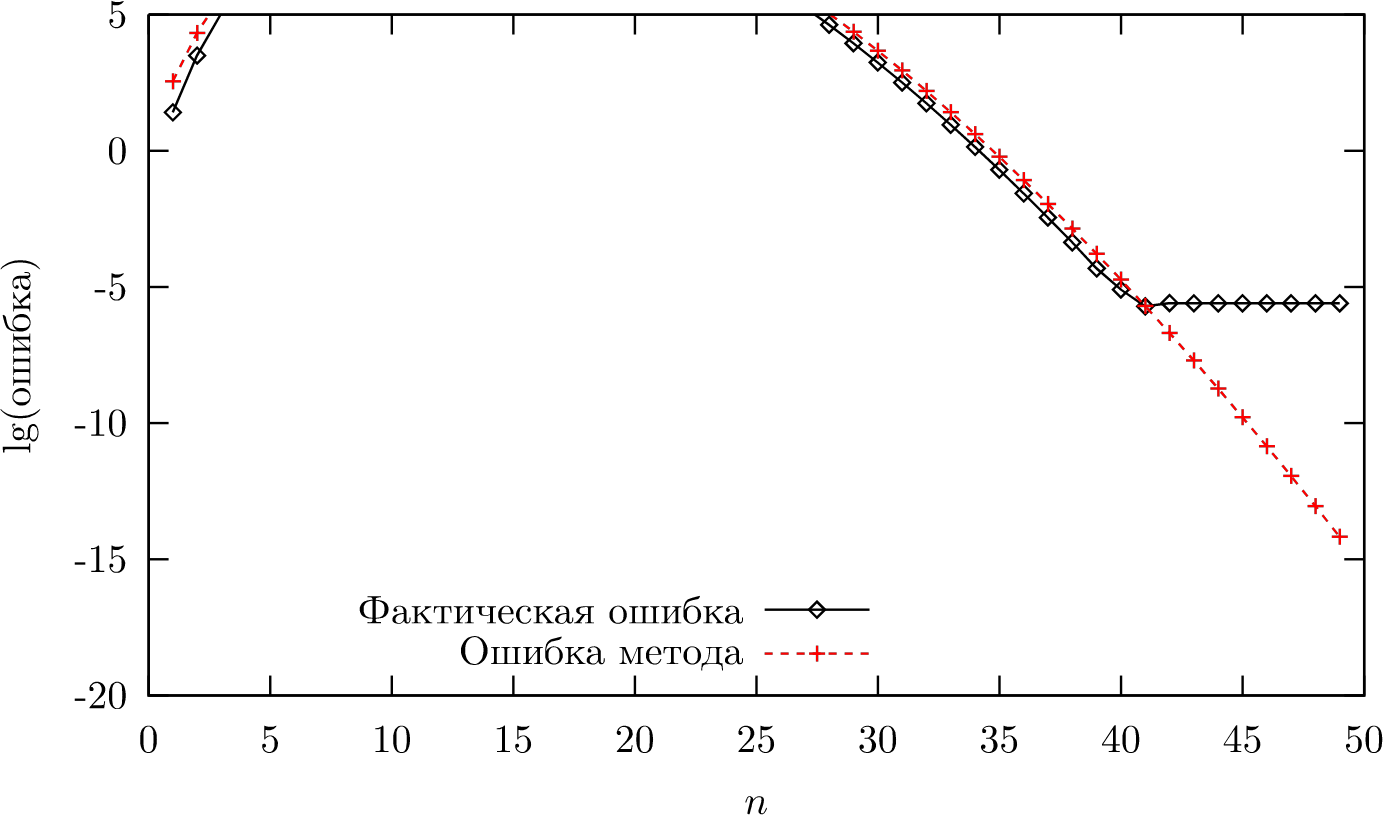
\includegraphics[height=0.4\textheight]{sine_17pi_2.png}
	\end{figure}

	Теперь ошибка перестает уменьшаться после 40 слагаемого и составляет уже $10^{-6}$.
	Определенно, данная ошибка может стать серьезной проблемой.
\end{frame}

\subsection{Особенности вычислительной техники}
\begin{frame}
\frametitle{Машинная арифметика}
	До сих пор все вычисления мы рассматривали в \emph{идеальной арифметике}, где все математические
	операции производятся \emph{абсолютно точно}. На практике, приходится иметь дело с машинной арифметикой,
	которая оперирует с \emph{приближенными} значениями чисел. Чаще всего, числа представлены в
	вычислительной технике в виде \emph{чисел с плавающей запятой} (floating-point values). Каждое число хранится
	в виде
	\[
	x = \pm s \cdot 2^e, \quad s = \overline{1.s_1s_2\dots s_K}
	\]
	где $1 \leqslant s < 2$ - мантисса, число с фиксированным количеством знаков после запятой, $e$ - экспонента или показатель степени,
	целое число. Поскольку целая часть мантиссы всегда равна 1, число значащих цифр в машинном представлении $x$ всегда совпадает с
	количеством знаков в мантиссе.
\end{frame}

\begin{frame}
\frametitle{Машинная арифметика в вычислениях}
	На практике, хранение чисел в форме с плавающей запятой приводит к хранению каждого числа с фиксированной относительной погрешностью.
	Например, в десятичной системе, если в мантиссе числа 5 значащих цифр (не считая первой единицы),
	то относительная погрешность хранения данного числа составляет $10^{-5}$
	\[
	1.23456 \cdot 10^{78} = (1.23456 \pm 0.000005) \cdot 10^{78}
	\]
	\[
	\bar X = 1.23456 \cdot 10^{78}, \,
	\Delta X = 0.00001 \cdot 10^{78}, \,
	\]
	\[
	\frac{\Delta X}{|\bar X|} = \frac{0.00001\cdot 10^{78}}{1.23456\cdot 10^{78}} = \frac{0.00001}{1.23456} < 10^{-5}
	\]
\end{frame}

\begin{frame}
\frametitle{Машинная арифметика в вычислениях}
	Аналогично, только с использованием двоичной, а не десятичной системы счисления, определяются
	относительные погрешности хранения стандартных числе с плавающей запятой
	\begin{itemize}
		\item тип single или float (32 бита) - мантисса имеет 23 значащих бита,
		относительная погрешность составляет $2^{-23} \approx 1.2 \cdot 10^{-7}$
		\item тип double (64 бита) - мантисса имеет 53 значащих бита,
		относительная погрешность составляет $2^{-53} \approx 1.1 \cdot 10^{-16}$
	\end{itemize}

	Действительное число $x$ в машинном представлении имеет вид
	\[
		x_\text{маш} = x (1 + \varepsilon(x)),
	\]
	где \[|\varepsilon(x)| \leqslant 2^{-K} |x|\]
\end{frame}

\begin{frame}
\frametitle{Вычислительные ошибки}
	\begin{figure}[ht!]
	\centering
	\includegraphics<1>[height=.4\textheight]{sine_pi_2.png}%
	\includegraphics<2>[height=.4\textheight]{sine_17pi_2.png}%
	\end{figure}
	Теперь понятно, что ошибка $10^{-16}$, которую мы получили при вычислении
	$\sin \frac{\pi}{2}$ --- это просто погрешность, с которой может быть представлен
	ответ в вычислительной технике.
	\pause
	\begin{block}{}
	Но как объяснить ошибку $10^{-6}$, которую мы получили, вычисляя $\sin \frac{17\pi}{2}$?
	\end{block}
\end{frame}

\begin{frame}
\frametitle{Ошибка округления. Оценка сверху}
	Так как округление до 16 значащих цифр\footnote{подразумеваем операции с double} происходит при \emph{каждой} операции,
	необходимо подсчитать суммарную ошибку округления всех слагаемых. Поскольку заранее неизвестно, в какую сторону происходит округление,
	необходимо сложить погрешности округления по модулю.
	\pause

	Оценим ошибку округления $S_n$.

	\[
	S_n = \sum_{k=0}^{n} (-1)^k\frac{x^{2k+1}}{(2k+1)!}
	\]
	\[
	\varepsilon_{\text{округ}} = \sum_{k=0}^{n} \left| 2^{-K}(-1)^k\frac{x^{2k+1}}{(2k+1)!} \right| =
	2^{-K}\sum_{k=0}^{n} \frac{x^{2k+1}}{(2k+1)!} \lesssim 2^{-K} \sh x
	\]
	Для $x = \frac{17\pi}{2} \approx 26.7$
	\[
	\varepsilon_{\text{округ}} \lesssim 2^{-K} \sh x = 2.1 \cdot 10^{-5}
	\]
\end{frame}

\begin{frame}
\frametitle{Ошибка округления. Оценка снизу}
{
	Итак, хотя исходный ряд был знакопеременным, и по модулю сумма ряда не превосходила единицы,
	отдельные слагаемые могли достигать весьма существенных	значений по модулю.

	\[
	\max_{k} \frac{x^{2k+1}}{(2k+1)!} \approx \frac{x^x}{x!} \approx \frac{x^x}{\sqrt{2\pi x}\left(\frac{x}{e}\right)^x} = \frac{e^x}{\sqrt{2\pi x}}
	\]
	\pause
	Возвращаясь к случаю $\sin \frac{17\pi}{2}$, $x \approx 26.7$
	\[
	\frac{e^x}{\sqrt{2\pi x}} = 3 \cdot 10^{10}.
	\]
	Погрешность округления только этого слагаемого $\varepsilon_{\text{округ}} = 2^{-53} \times 3 \cdot 10^{10} \approx 3.3 \cdot 10^{-6}$,
	что вполне соответствует фактической ошибке при вычислении $\sin \frac{17\pi}{2}$.
}
\end{frame}

\subsection{Вывод}
\begin{frame}
\frametitle{Вывод}
{
	Практически все прикладные задачи , которые приходится решать в рамках вычислительной математики, невозможно решить точно.
	Этому препятствует два основных источника погрешности --- неточные(приближенные) методы и неидеальная(машинная) арифметика.
	Ошибке метода соответствует погрешность решения задачи в идеальной арифметике (в которой все действия выполняются точно).
	В ошибку округления входят погрешности всех вычислений при реализации данного метода.
}
\end{frame}

\section{Численное дифференцирование}
\subsection{Вычисление производной}
\begin{frame}
\frametitle{Производная}
	\begin{block}{Задача}
	Допустим, задана функция $f(x)$, то есть мы можем вычислить ее значение в любой точке $x$.
	Как вычислить ее производную в заданной точке $x_0$?
	\end{block}
	\pause
	Вспомним определение производной
	\[
	f'(x_0) = \lim_{\Delta x \rightarrow 0} \frac{f(x_0+\Delta x) -
	f(x_0)}{\Delta x}
	\]
	\begin{block}{Вопрос}
	Какие еще определения производной Вы знаете?
	\end{block}
\end{frame}

\subsection{Конечные разности}
\begin{frame}
\frametitle{Численный метод}
	\[
	f'(x_0) = \lim_{\Delta x \rightarrow 0} \frac{f(x_0+\Delta x) - f(x_0)}{\Delta x}
	\]
	Поиск предела, так же как и суммирование бесконечной суммы, является нетривиальной операцией.

	\pause
	Заменим предел значением отношения при некотором маленьком значении $\Delta x = h > 0$.

	\[
	f'(x_0) \approx \frac{f(x_0+h) - f(x_0)}{h}
	\]
	Такие выражения называются в вычислительной математике \emph{конечными
	разностями}.
\end{frame}

\begin{frame}
\frametitle{Ошибка метода}
	В первую очередь, нас интересует ошибка метода, которая возникает в результате замены предела
	конечной разностью. Здесь нам снова поможет формула Тейлора. Разложим $f(x)$ в окрестности
	точки $x = x_0$.

	\[
	f(x) = f(x_0) + (x-x_0) f'(x_0) + \frac{(x-x_0)^2}{2} f''(\xi), \quad \xi \in [x_0,x]
	\]
	\pause
	Подставляя $x = x_0 + h$,
	\[
	f(x_0 + h) = f(x_0) + h f'(x_0) + \frac{h^2}{2} f''(\xi), \quad \xi \in [x_0,x_0+h]
	\]
\end{frame}

\begin{frame}
\frametitle{Ошибка метода}
	\[
	f(x_0 + h) = f(x_0) + h f'(x_0) + \frac{h^2}{2} f''(\xi), \quad \xi \in [x_0,x_0+h]
	\]

	Группируем и делим на $h$

	\[
	\frac{f(x_0 + h) - f(x_0)}{h} - f'(x_0) = \frac{h}{2} f''(\xi)
	\]

	\[
	\varepsilon_{\text{метод}} = \left|\frac{f(x_0 + h) - f(x_0)}{h} - f'(x_0) \right| = \left |\frac{h}{2} f''(\xi) \right | \leqslant \frac{M_2 h}{2}
	\]

	Чем меньше $h$, тем меньшим оказывается погрешность метода. Погрешность метода линейно зависит от $h$.
\end{frame}

\subsection{Метод неопределенных коэффициентов}
\begin{frame}
\frametitle{Метод неопределенных коэффициентов}
	Будем искать другие способы вычисления производной. Допустим, мы хотим построить наиболее
	точный метод для вычисления производной, который бы использовал значения функции в трех точках ---
	в $x_0, x_0+h$ и $x_0-h$.

	Некоторые соображения о том, в каком виде следует искать требуемый метод дают свойства оператора дифференцирования.
	Известно, что операция дифференцирования линейна, т.е.
	\[
	(\alpha f + \beta g)' = \alpha f' + \beta g'
	\]
	Вполне логично искать \emph{линейную} формулу дифференцирования, т.е. такую, в которую значения дифференцируемой функции входят
	\emph{линейно}
\end{frame}

\begin{frame}
\frametitle{Метод неопределенных коэффициентов}
	Запишем линейную функцию от $f(x_0), f(x_0+h), f(x_0-h)$ в виде линейной комбинации с неопределенными коэффициентами
	\[
	f'(x_0) \approx \frac{\alpha f(x_0-h)  + \beta f(x_0) + \gamma f(x_0+h)}{h}
	\]
	За счет надлежащего выбора $\alpha, \beta, \gamma$ добьемся максимального совпадения левой и правой части равенства.

	\pause
	Потребуем совпадения максимального количества членов в представлении в виде формулы Тейлора в точке $x_0$ левой и правой частей.
	\begin{block}{Замечание}
	Здесь делается предположение, что у функции $f(x)$ существует достаточное количество производных в точке $x_0$.
	Необходимо иметь в виду, что если функция $f(x)$ не имеет всех необходимых производных, погрешность метода может увеличиваться.
	\end{block}
\end{frame}

\begin{frame}
\frametitle{Формула Тейлора}
	\[
	f'(x_0) \approx \frac{\alpha f(x_0-h)  + \beta f(x_0) + \gamma f(x_0+h)}{h}
	\]
	Представляя значения в крайних точках с помощью формулы Тейлора
	\[
	f(x_0 \pm h) = f(x_0) \pm h f'(x_0) + \frac{h^2}{2} f''(x_0) \pm \frac{h^3}{6} f'''(\xi_{1,2})
	\]
	\[
	\xi_1 \in [x_0-h, x_0],\xi_2 \in [x_0, x_0+h]
	\]
	\[
	f'(x_0) \approx \frac{\alpha + \beta + \gamma}{h} f(x_0) + (\gamma - \alpha) f'(x_0) + (\alpha+\gamma) \frac{h}{2}f''(x_0) + R
	\]
	\[
	R = \frac{h^2}{6}\Big(\gamma f'''(\xi_2) - \alpha f'''(\xi_1)\Big)
	\]
\end{frame}

\begin{frame}
\frametitle{Определение коэффициентов}
	После исключения значений функции в крайних точках, приближенное равенство приобретает вид
	\[
	f'(x_0) \approx \frac{\alpha + \beta + \gamma}{h} f(x_0) + (\gamma - \alpha) f'(x_0) + (\alpha+\gamma) \frac{h}{2}f''(x_0) + R
	\]
	\[
	R = \frac{h^2}{6}\Big(\gamma f'''(\xi_2) - \alpha f'''(\xi_1)\Big)
	\]
	Потребуем, чтобы $\alpha + \beta + \gamma = 0, (\gamma - \alpha) = 1, (\alpha+\gamma) \frac{h}{2} = 0$.
	Искомые значения $\gamma = -\alpha = \frac{1}{2}, \beta = 0$.
	При этом равенство превратится в
	\[
	f'(x_0) \approx f'(x_0) + R
	\]
	Добавка $R$ как раз будет ошибкой метода.
	\[
	\varepsilon_{\text{метод}} = |R| = \frac{h^2}{6} \frac{1}{2}|f'''(\xi_2) + f'''(\xi_1)| \leqslant \frac{h^2}{6} M_3
	\]
\end{frame}

\subsection{Порядок метода}
\begin{frame}
\frametitle{Формулы дифференцирования 1-го и 2-го порядков}
	Формула $f'(x_0) \approx \frac{f(x_0+h) - f(x_0)}{h}$ называется формулой односторонней разности, а
	$f'(x_0) \approx \frac{f(x_0 + h) - f(x_0 - h)}{2h}$ --- формулой центральной разности. Важное различие этих формул заключается
	в разной зависимости ошибки метода от $h$. Для односторонней разности эта зависимость линейная
	$\varepsilon_{\text{метод}} \leqslant \frac{M_2 h}{2}$, в то время как для центральной --- квадратичная
	$\varepsilon_{\text{метод}} \leqslant \frac{M_3 h^2}{6}$.
	\pause

	Говорят, что формула односторонней разности имеет \emph{первый порядок аппроксимации},
	а центральной - \emph{второй порядок аппроксимации}
\end{frame}

\begin{frame}
\frametitle{Проверка}
	Проверим, действительно ли зависимость ошибки имеет такой характер для каждой из формул. Рассчитаем $\sin'1 = \cos 1$

	\begin{figure}%
	\centering
	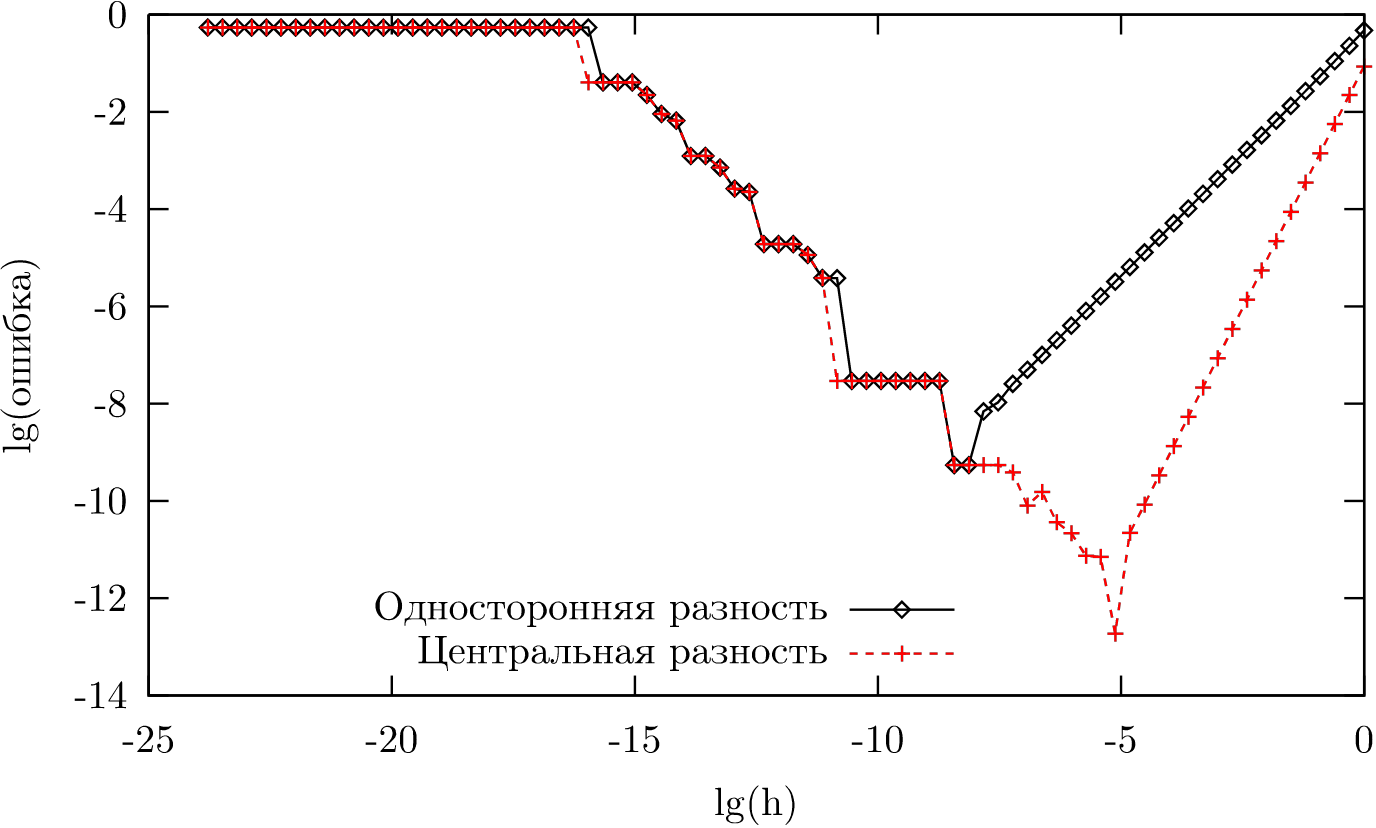
\includegraphics[height=0.5\textheight]{diff.png}%
	\end{figure}

	Оказывается, поведение ошибки имеет такой характер только при сравнительно больших $h$. Для односторонней разности при $h > 10^{-8}$,
	а для центральной --- при $h > 10^{-5}$.
\end{frame}

\begin{frame}
\frametitle{Вычислительные погрешности}
	Проще всего объяснить постоянное значение ошибки при использовании $h < 10^{-16}$. При данном значении величины
	$x_0+h = 1+h$ и $x_0-h = 1-h$ округляются до $1$, при этом в числителе обеих формул стоит тождественный ноль, 
	хотя реальное значение производной ненулевое.
	\pause

	Учтем теперь, что значения $f(x_0), f(x_0 + h)$ сами по себе могут содержать
	ошибки (например, из-за машинного хранения или вычисления по приближенному
	алгоритму):
	\[
	f'(x_0) \approx \frac{(f(x_0+h) \pm \Delta f) -(f(x_0) \pm \Delta f)}{h}
	\]
	\[
	\varepsilon_{\text{выч}} \leqslant \frac{2\Delta f}{h}
	\]
	Если $\Delta f$ обусловлена только ошибкой машинного представления, то
	\[
	\Delta f \lesssim 2^{-K} |f(x_0)|, \qquad \varepsilon_\text{выч} \leqslant
	2\frac{2^{-K}|f(x_0)|}{h}
	\]
\end{frame}

\begin{frame}
\frametitle{Оптимальное значение h}
	Итак, при слишком маленьких значениях $h$ основной вклад в ошибку дает
	именно вычислительная погрешность, которая растет с уменьшением $h$, а
	при слишком больших становится значительной ошибка метода. Найдем оптимальное значение
	$h$, при котором сумма обеих ошибок имеет минимальную величину.
	\pause

	\only<1-2>{Для односторонней разности
	\[
	\varepsilon_{\text{сумм}} =
	\varepsilon_{\text{выч}} +
	\varepsilon_{\text{метод}} =
	\frac{2\Delta f}{h} + \frac{M_2 h}{2}
	\]
	\[
	h_\text{опт} = 2\sqrt{\frac{\Delta f}{M_2}},\text{ при этом }
	\varepsilon_{\text{сумм}} = 2\sqrt{M_2 \Delta f}
	\]
	Для проверки подставим $M_2 = 1, \Delta f=10^{-16}$, тогда
	\[h=2 \cdot 10^{-8},  \quad \varepsilon_{\text{сумм}} = 2 \cdot 10^{-8}\]}%
	\only<3>{Для центральной разности
	\[
	\varepsilon_{\text{сумм}} =
	\varepsilon_{\text{выч}} +
	\varepsilon_{\text{метод}} =
	\frac{2\Delta f}{2h} + \frac{M_3 h^2}{6}
	\]
	\[
	h_\text{опт} = \sqrt[3]{\frac{6\Delta f}{M_3}},\text{ при этом }
	\varepsilon_{\text{сумм}} =	\frac{3}{2} \sqrt[3]{\frac{M_3 \Delta f^2}{3}}
	\]
	Для проверки подставим $M_3 = 1, \Delta f = 10^{-16}$, тогда
	\[h \approx 6.7 \cdot 10^{-6},  \quad \varepsilon_{\text{сумм}} \approx 2.2 \cdot
	10^{-11}\]}%
\end{frame}

\begin{frame}
\frametitle{Вывод}
	Важно отметить, что при использовании формулы второго порядка удалось получить меньшую суммарную погрешность
	не выходя за пределы той же машинной точности что и в формуле первого порядка, то есть только за счет выбора
	более качественного метода.
	\pause

	Однако, не стоит забывать что функция, которую мы дифференцировали была достаточное
	число раз (а именно 3 раза) непрерывно дифференцируема. Если формулу второго порядка применять
	к функции, у которой, например, $M_3 = \infty$, но $M_2 < \infty$, то оценка ошибки метода имела бы
	такой же вид, как у формулы односторонней разности 1го порядка. В этом случае выигрыш был бы совсем
	незначительным.
\end{frame}

\begin{frame}[plain]
  \begin{center}
  {\Huge Спасибо за внимание!}
  \vspace{8ex}

  Цыбулин Иван

  e-mail: \colorhref{mailto:tsybulin@crec.mipt.ru}{tsybulin@crec.mipt.ru}
  \end{center}
\end{frame}

\end{document}
